\documentclass[12pt]{article}
\title{Sabotage with Chaos }
\author{林橋毅 111502563}
\usepackage[UTF8]{ctex}
\usepackage{graphicx} %插入图片的宏包
\usepackage{float} %设置图片浮动位置的宏包
\usepackage{caption}
\usepackage{subfigure} %插入多图时用子图显示的宏包
\usepackage{algorithm}
\usepackage{cite}
\usepackage{algpseudocode}
\usepackage{amsmath}
\usepackage{graphics}
\usepackage{epsfig}
\usepackage{amssymb}
\usepackage{bm}
\usepackage{hyperref}
\usepackage{graphicx}
\newtheorem{definition}{Definition}

\begin{document}
	\captionsetup[figure]{labelfont={bf}, labelformat={default}, labelsep=period,name={Fig.}}
	\maketitle
	
	\part{Introduction}
	本題是 UVa 10480 Sabotage,簡單來說,給定一個連通圖,要將這張圖分成兩個連通分塊(Connected component),其中這兩個連通分塊分別包含 s 跟 t,也就是說 s 跟 t 不能在同一個連通分塊中,也等同於把 s 跟 t 分開的意思,要將圖分開勢必得破壞邊,但要怎麼切邊才能使拿掉的邊權重總和最小,這是經典的 Minimum cut 問題。\\
	
	標準的做法是使用 Max-Flow 的演算法並利用 Max-Flow Min-Cut Theorem 解決這個問題。但因為 Max-Flow 的演算法都較難實作,所以本次專題使用  Randomize 的做法,用隨機合併邊的方法,得到候選答案,並執行多次找到最好的解法提升答對率。

	本篇將介紹實作該演算法的方式並且探討該演算法的正確率以及執行速度。
	
	\part{Method}
	
	\section{Flow}
	本題我使用課堂中報告的 Edmonds–Karp 算法解決這題。
	不斷使用 BFS 尋找最短的擴增路徑,並且記錄剩餘的流量,直到找不到為止,最多只要找 VE 次就可以找到最大流。
	
	\begin{algorithm}[H]
		\caption{Edmonds-Karp }
		\begin{algorithmic}
			\State Initialize the flow
			\While{BFS-ShortestPath == true}
				\State Update the flow of each edge
			\EndWhile
		\end{algorithmic}
	\end{algorithm}

	\begin{algorithm}[H]
		\caption{bfs-ShortestPath}
		\begin{algorithmic}
			\State Queue <- s
			\While{!Queue.empty()}
				\State i <- Queue.front() ; Queue.pop();
				\For{each vertex}
					\If{the vertex is not visited}
						\State Calculate bottleneck flow
						\State Find shortest path
						\State Queue.push(vertex)
						\State return the flow
					\EndIf
				\EndFor
			\EndWhile
			\State return false; // 找不到了
		\end{algorithmic}
	\end{algorithm}
	\section{Randomized}
	這個演算法相似於 Karger's algorithm,但這是解決全域 minimum cut 問題,但我們要解決的是 s-t cut。
	
	這個方法的核心是不斷地合併隨機一條邊(但這條邊的端點不可同時是 s 與 t),將這條邊的兩端點合併成一個 supernode,重複執行合併直到只剩下兩個點後,該兩點(supernode)將各別包含 s 和 t,這兩點之間所連接的邊權重和將會是我們的候選答案,執行多次後將候選答案中最小的輸出做為答案。因為很好實作也很快,只要重複執行足夠次後將可以大大提升正確率。 
	
	實作中我使用並查集(Disjoined set)儲存被合併的邊。
	
	\begin{algorithm}[H]
		\caption{Randomized}
		\begin{algorithmic}
			\State times = 1000 // number of execute
			\State vertices =  Number of vertices 
			\While{times != 0}
				\While{vertices > 2}
					\State e = Random select a edge 
					\If{not in the same supernode and not connect s and t }
						\State combine the edge
						\State vertices -= 1
					\EndIf
					\State times -= 1
				\EndWhile
			\EndWhile
		\end{algorithmic}
	\end{algorithm}
	
	\part{Experiment}
	\section{Test Data \& Description}
	
	本次專題,我使用 \href{https://github.com/ifsmirnov/jngen}{jngen.h} 這個套件幫我快速生成測試資料,這個套件可以快速的讓我生成我要的 Graph。
	我的測試資料是隨機的 無向無環連通圖,並且編譯成 lib.o 方便連結。\\
	
	
	本次的解法是 maxFlow.cpp 以及 randomizelcpp,並且 env01.zip、env02.zip、env03.zip,分別依序是下列的實驗所使用的程式碼以及生成器,編譯時連接 lib.o 即可使用。另外 Analysis\_Flow\_prj.ipyb 是製作分析圖表的程式。
	\section{UVa Online judge}
	
	檢驗原本使用Edmend karp 解 Max Flow 問題在官方 UVa Online Judge 的正確性。
	因為原題目的測資小而且演算法也算有效率,可以看到執行時間非常快不到 0.01 秒就通過測試。
	
	\section{Accuracy}
	
	為了測試答案正確率,固定變因後比較答案與平均執行時間,我選擇與原題相似的條件,以下是測資的資訊:
	\begin{description}
		\item[1.] 測試資料總數:10000
		\item[2.] 點數: 50
		\item[3.] 邊數:500
		\item[4.] 權重範圍:1 $\sim$ 40000000
	\end{description}
	
	以下是本次測試的結果:
	\begin{table}[htbp]
		\center
		\caption{隨機演算法正確率與執行時間}
		\resizebox{\linewidth}{!}{
		\begin{tabular}[h]{ | c | c | c | c | c | c | } 
			\hline 
			& Max-Flow 解法(正確答案) & 隨機合併 50 次  & 隨機合併 500 次 & 隨機合併 1000 次 & 隨機合併 2500 次 \\
			\hline
			正確率 & 100 \% & 99.798995 \% &  100 \% & 100 \% & 100 \% \\
			\hline
			平均執行時間(ms)& 0.252863  & 1.7181518 & 16.304765 & 32.489433  & 83.289581 \\
			\hline
		\end{tabular}}
	\end{table}
	
	
	\section{Complexity}
	
	為了測試兩個演算法的執行時間,我設計了兩組實驗,分別是
	
	\begin{description}
		\item[1.] 固定稀疏程度 50 \%,測試點數由 2 到 200  的執行時間,其中測試隨機演算法的執行次數為 $V^2$ 與 $V$ 次
		\item[2.] 固定點數為 50,測試稀疏程度由 5\% 到 100 \% 的執行時間,其中固定隨機演算法的執行次數為 2500  與 50 次
	\end{description}
	兩組實驗為了不使用 long long 儲存 cost 將邊權重設為 1 $\sim$ 5000。 \\
	
	定義:一張圖有 V 個點、E 條邊的稀疏程度為 $\frac{E}{\frac{V*(V-1)}{2}} * 100 \%$  \\
	
	本次之所以使用稀疏程度作為實驗變因的原因是,本演算法的時間複雜度會同時受到點跟邊的數量影響。
	但如果固定點數增加邊數會受到點數的影響造成無法完美固定變因,故我認為使用稀疏程度較能比較演算法的執行時間。
	
	
	\subsection{Result}
	
	\paragraph{固定稀疏程度 50 \%} \leavevmode \\
	
	當固定稀疏程度並增加點的數量,每組資料生成五個測資並在最後將其平均,邊的數量將隨著點的數量成長,在隨機演算法中不管做 V 次 還是做 $V^2$ 次的執行時間都相對標準的 Max-Flow 解法表現要差,但可以觀察到當隨機做 V 次時的複雜度與標準的算法能夠在相同的 Order(從程式碼分析亦同),而根據上一節的結果又可以看到當我們做 V 次時的正確率有 99 \% 左右,所以在相同時間複雜度時隨機演算法能有接近 99 \% 的好表現。 \\
	
	雖然有著相同的複雜度,但有可能因為隨機數產生會耗費多次時間,若可以採用更高效率的隨機數產生器也許能再更進一步加速隨機演算法的執行時間。
	
	\begin{figure}[H]
		\centering
		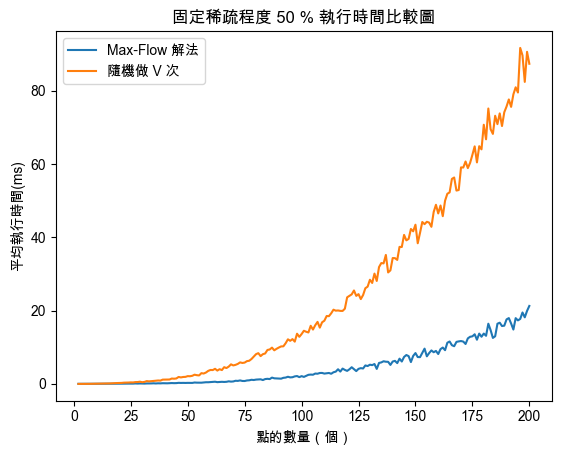
\includegraphics[width=0.8\textwidth]{img/img0}
		\caption{固定稀疏程度時 Max-Flow 與 隨機執行 V 次的執行時間比較圖}
		\label{Fig.0}
	\end{figure}

	\begin{figure}[H]
		\centering
		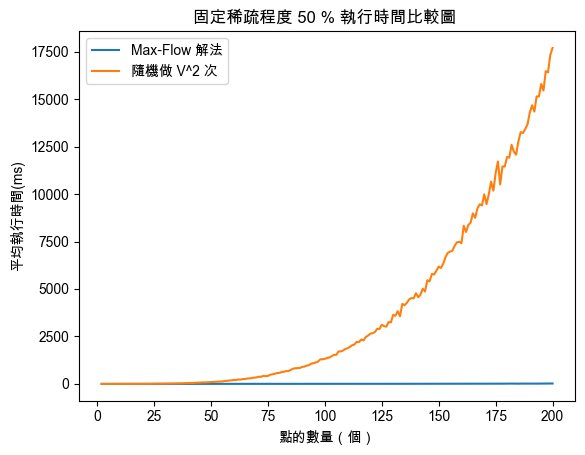
\includegraphics[width=0.8\textwidth]{img/img1}
		\caption{固定稀疏程度時 Max-Flow 與 隨機執行 $V^2$ 次的執行時間比較圖}
		\label{Fig.1}
	\end{figure}
		\begin{figure}[H]
		\centering
		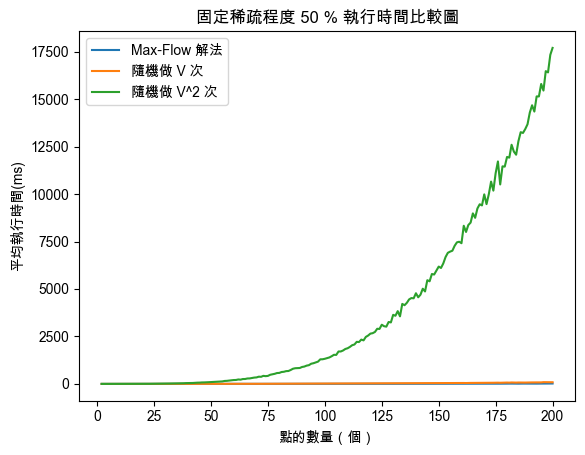
\includegraphics[width=0.8\textwidth]{img/img2}
		\caption{固定稀疏程度時執行時間比較圖}
		\label{Fig.2}
	\end{figure}

	\paragraph{固定點數為 50 點}  \leavevmode \\
	
	在這個實驗我們固定點並增加稀疏程度,同樣一個資料生成五個測資並做平均,邊的數量隨之增加,圖將越來越稠密、越來越接近 Complete Graph,我們測試了在固定點數量時的執行時間。\\
	
	同樣可以看到隨機演算法執行時間慢於標準的 Max-Flow 演算法的執行時間,也同樣的在執行 V 次時可以與標準解法有類似的複雜度,做 $V^2$ 次差於標準解法。
	
	\begin{figure}[H]
		\centering
		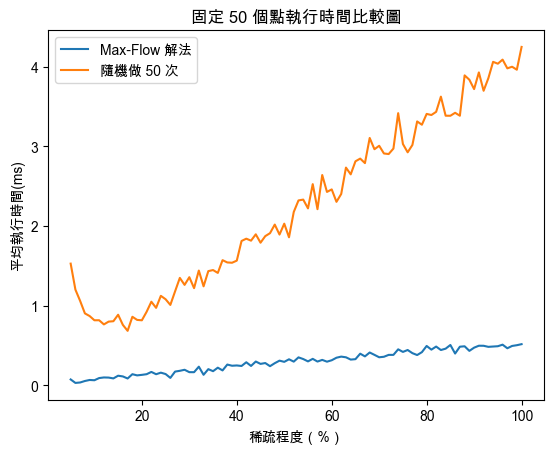
\includegraphics[width=1\textwidth]{img/img3}
		\caption{固定 50 個點時 Max-Flow 與 隨機執行 50 次的執行時間比較圖}
		\label{Fig.3}
	\end{figure}	

	\begin{figure}[H]
		\centering
		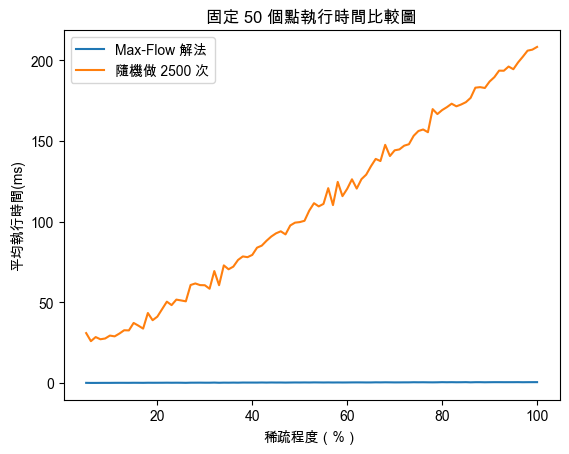
\includegraphics[width=1\textwidth]{img/img4}
		\caption{固定 50 個點時 Max-Flow 與 隨機執行 2500 次的執行時間比較圖}
		\label{Fig.4}
	\end{figure}
	
	\part{Conclusion \& Reflection}	
	本篇實驗了使用隨機合併邊的演算法求解 Max-Flow Min-Cut 問題的正確性以及速度,在隨機演算法執行 V (點的數量)次時就可以有很好的正確性,但即便執行 V 次時執行速度仍然比標準的 Max-Flow 解法還要慢,但這個演算法非常好實作,觀念也很容易理解,這成為這個演算法非常大的優點。 \\
	
	透過這次專題,讓我開啟很多近似演算法的想法,在競賽上可能不是個好方法,但在實務上也許因為他的好操作性,可以作為不錯的驗證想法的演算法。\\
	
	但因為我使用得是 random.h 內的內建隨機數產生器,我們知道這是一個不完美的隨機數產生器,期望未來能夠藉此分析隨機數產生器的隨機性,或者更完美或者更高效的隨機數產生器,例如:MT19937、量子隨機數產生器等等,有可能能夠增加準確性或分析參考性。
\end{document}